% !TeX root = ../main.tex

\chapter{Theoretical Background}\label{chapter:theoretical_background}

\section{Natural Language Processing}
\paragraph{Natural language processing }(NLP) is a subfield of computer science which focuses on, as implied by the name, processing of human (natural) languages. NLP enables us to make use of copious knowledge that is expressed in natural language. \parencite{ai_nlp} 


In this section we will be taking a look at some NLP concepts that are relevant to us. 
Most of the knowledge provided here is based on \parencite{nlp}.
We will start with regular expressions, powerful tools able to catch text patterns. 
Then we will be looking at information extraction from natural language. 
Finally, we will finish this chapter on dialog systems and chatbot.

\subsection{Regular Expressions}
\paragraph{A regular expression}is formally defined as an algebraic notation that represents a specific set of strings.
However, this representation is not explicit. 
Regular expressions denote textual patterns which are able to produce implicit sets.
These patterns are useful for searching in text.
A regular expression search function finds every instance of text in the corpus that belongs to the pattern's implicit set.
These instances are said to be 'matched' by the pattern.

Regular expressions are supported in every computer language, word processor and text processing tool. 
However, there may be differences in how they treat certain expressions. 
As the knowledge provided here is based on \parencite{nlp_re}, we will be treating expressions as they are shown there.
Another thing to keep in mind is that this is not a comprehensive guide for regular expression. 
We will be looking at basics and some more complex operators we need for our specific problem. 

\subsubsection{Basic Regular Expression Patterns}
Simplest regular expressions are sequences of characters. 
For example \texttt{snack} matches any string that contains the sequence 'snack'. 
Here are some examples that would be matched by this regular expression:\\
"I just had a small \underline{snack}."\\
"His username was 123\underline{snack}o."\\
As we see, this regular expression only searches for the sequence 'snack'.
Whether the found sequence actually is a word or not is irrelevant.

The period \texttt{.} is treated as a special character: the wildcard.
It matches any character, so for example \texttt{r.n} matches:\\
"I \underline{ran} 5k today."\\
"You better \underline{run}."\\
Another special character is the question mark: \texttt{?}
Adding a question mark after an element makes the element optional. 
For example, \texttt{hours?} matches:\\
"The \underline{hour} arm of the clock was missing."\\
"I have been waiting for you for \underline{hours}."\\
Special characters can also be used as regular characters.  
We just need to put a backslash \texttt{\textbackslash} before the special character.
For example, \texttt{Inc\textbackslash.} matches:\\
"Monsters \underline{Inc.} was a great movie."

\begin{table}[htbp]
  \caption[Regular Expression Basics]{Regular Expression Basics}\label{tab:re_basic}		
  \centering
  \begin{tabular}{l l l}
    Regular Expression&Match&Example\\ \toprule
    \texttt{duck}&'duck'&\underline{duck}\\ \hline
    \texttt{r.ck}&'r' and 'ck' with any character in between&\underline{rock}, \underline{rack}\\ \hline
    \texttt{minutes?}&'minute' or 'minutes'&\underline{minute},\underline{minutes}\\ \hline
    \texttt{\textbackslash?}&'?'&How\underline{?}\\ \hline
  \end{tabular}
\end{table}

\subsubsection{Square Brackets, Range and Negation}

It is important to note that regular expressions are case sensitive, so \texttt{meal} matches the first example, but not the second:\\
"We had a tasty \underline{meal}."\\
"Meal is ready."\\
This problem is solved by the use of square brackets:\texttt{[]}.
Square brackets signify a disjunction between the characters inside. 
So \texttt{[Mm]} means either 'M' or 'm' and \texttt{[Mm]eal} matches both examples:\\
"We had a tasty \underline{meal}."\\
"\underline{Meal} is ready."\\
Square brackets can be used for regular expression that match any digit \texttt{[1234567890]} or any letter \texttt{[abcdefghijklmnopqrstuvwxyz]}.
However, for such common disjunctions we can also use the dash \texttt{-} operator.
Dash operator denotes a range: \texttt{[0-9]} matches any digit between '0' and '9'.
\texttt{[a-z]} and \texttt{[A-Z]} match any lowercase letter and any uppercase letter, respectively.

Another use of square brackets is negation. 
When a caret \texttt{\^} is the first character inside a bracket, any character other than the ones inside the brackets is matched.
\texttt{[\^{}ab]} matches any character that is not 'a' or 'b'. 
\texttt{[\^{}0-9]} matches any character that is not a digit.

It is important to note that when used outside of these contexts, both dash \texttt{-} and caret \texttt{\^} have different meanings.
Outside of the brackets, dash operator is treated as a character. 
When the caret occurs in the brackets after the first character, it is also treated as a character.
For example, \texttt{0-9} matches the first sentence but not the second:\\
"Please enter a value between \underline{0-9}."\\
"This course is worth 8 ECTS credits."

There are some shorthands for commonly used ranges or disjunctions.
\texttt{\textbackslash d} is equivalent to \texttt{[0-9]} and matches any digit. 
\texttt{\textbackslash s} matches any whitespace. 

\begin{table}[htbp]
  \caption[Regular Expression Square Brackets]{Use of Square Brackets}\label{tab:re_sb}		
  \centering
  \begin{tabular}{l l l}
    Regular Expression&Match&Example\\ \toprule
    \texttt{[Ss]nack}&'Snack' or 'snack'&\underline{Snack},\underline{snack}\\ \hline
    \texttt{[0-9]}&Any digit&\underline{5} missed calls!\\ \hline
    \texttt{[\^{}abc]}&Any character that is not 'a','b' or 'c'&ca\underline{r}b\\ \hline
    \texttt{[3\^{}2]}&'3','\^{}', or '2'&n\underline{\^{}}1 equals n\\ \hline
    \texttt{\textbackslash d}&Any digit&\underline{5} missed calls!\\ \hline
    \texttt{\textbackslash s}&Any whitespace&5\underline{ }missed\underline{ }calls!\\ \hline
  \end{tabular}
\end{table}

\subsubsection{Disjunction and Anchors}

Now, with the help of square brackets, we are capable of basic disjunction between characters. 
But what if we need a pattern that matches either 'meal' or 'snack'?
\texttt{[mealsnack]} would not work as square brackets denote character level disjunction. 
What we need here is the pipe symbol \texttt{|}, the disjunction operator.
\texttt{snack|meal} matches both of the following examples:\\
"I need a \underline{snack}."\\
"When was your last \underline{meal}"\\
Next, we have the anchors: special characters that can specify locations in text.
For example, the caret operator \texttt{\^{}} when used outside of brackets specify the start of a line.
The dollar sign \texttt{\$} specifies the end of a line.
So \texttt{\^{}I|\textbackslash?\$} matches any sentence that either starts with I or ends with a question mark:\\
"\underline{I} thought we were gonna eat together."\\
"Are you available for lunch \underline{?}\\
We have two more anchors that we can make use of:
\texttt{\textbackslash b} to match word boundaries and \texttt{\textbackslash B} to match non-boundaries.
For example, \texttt{\textbackslash bsnack\textbackslash b} matches the first sentence, but not the second:\\
"I just had a small \underline{snack}."\\
"His username was 123snacko."\\
To use these anchors, it is important to understand what a word means.
In terms of regular expressions, a word is defined as any sequence of digits, letters or underscores.
So \texttt{\textbackslash bap\textbackslash b} would match 'A\$\underline{ap}'.
As \$ is neither a digit or a letter or underscore, it is treated as a word boundary.

\begin{table}[htbp]
  \caption[Regular Expression Disjunction and Anchors]{Disjunction and Anchors}\label{tab:re_da}		
  \centering
  \begin{tabular}{l l l}
    Regular Expression&Match&Example\\ \toprule
    \texttt{eat|ate}&'eat' or 'ate'&I just \underline{ate}.\\ \hline
    \texttt{\^{}\textbackslash .}&Any character at the start of a line&\underline{I} just ate.\\ \hline
    \texttt{\textbackslash .\$}&Any character at the end of a line&I just ate\underline{.}\\ \hline
    \texttt{\textbackslash b59\textbackslash b}&'59' between word boundaries&It costs \$\underline{59}.99.\\ \hline
    \texttt{\textbackslash B59\textbackslash B}&'59' between non-boundaries&It costs \$2\underline{59}9.\\ \hline
  \end{tabular}
\end{table}

\subsubsection{Kleene Operators, Grouping and Precedence}

There are cases where we need to match repetitive patterns.
For example, we might want to match any 'hey' with an arbitrary amount of 'y's.
To do this, we can use the Kleene Star \texttt{*}.
Kleene star means "0 or more occurrences of the preceding element".
This means \texttt{y*} matches '','y','yy' and any other number of 'y' characters.
So in order to match any 'hey' with an arbitrary amount of 'y's, we would use \texttt{heyy*}.
This use, however, is so common that we have another operator for it: the Kleene Plus \texttt{+}.
Kleene Plus means "1 or more occurrences of the preceding element".
So \texttt{heyy*} and \texttt{hey+} are functionally equal.

But what if we need to match a phrase such as as 'hahaha', which consists of an arbitrary number of 'ha's?
\texttt{ha+} would not work, because the Kleene operator works on the preceding element.
So how can we set 'ha' as the preceding element?

This is where grouping comes into play.
In regular expressions, grouping is done by wrapping a phrase in parentheses. 
From then on, the phrase inside the parentheses is treated as a singular entity by operators outside the parentheses.
\texttt{(ha)+} matches any 'ha', 'haha' and any number of repetitions of the phrase 'ha'.

Grouping also comes in handy when using the disjunction operator.
For example, let's assume we need a regular expression that matches 'hour', 'minute', 'hours' and 'minutes'.
We ca not use \texttt{hour|minutes?}, because the disjunction is between \texttt{hour} and \texttt{minutes?}
This is because the \texttt{?} is evaluated first, then the sequences and only then the disjunction. 
Instead, we can use \texttt{(hours|minute)s?}. 
This expression works since the parentheses are evaluated before all the other operators.

The collection of rules determining which operator is evaluated first is called the operator precedence hierarchy.
An operator x is said to have precedence over another operator y, if x is to be evaluated before y.
Regular expression operator precedence hierarchy is as follows, from highest precedence to lowest precedence:

\begin{table}[htbp]
  \caption[Regular Expression Operator Precedence Hierarchy]{Regular Expression Operator Precedence Hierarchy}\label{tab:re_oph}
  \centering
  \begin{tabular}{l l l}
    Parentheses&\texttt{()}&\\ \hline 
    Counters&\texttt{* + ?}&\\ \hline 
    Sequences and anchors&\texttt{seq \^{}I \textbackslash.\$}&\\ \hline 
    Disjunction&\texttt{|}&\\ \hline 
  \end{tabular}
\end{table}


\begin{table}[htbp]
  \caption[Regular Expression Kleene Operators and Grouping]{Regular Expression Kleene Operators and Grouping}\label{tab:re_kog}
  \centering
  \begin{tabular}{l l l}
    Regular Expression&Match&Example\\ \toprule
    \texttt{b*}&0 or more repetitions of 'b'&aaa\underline{bbb}\\ \hline
    \texttt{a+}&1 or more repetitions of 'a'&\underline{aaa}bbb\\ \hline
    \texttt{(ab)+}&1 or more repetitions of 'ab'&aa\underline{ab}bb\\ \hline
  \end{tabular}
\end{table}

\subsubsection{Capture Groups}

Let's assume we have a list of names and we want to make sure all the names occur only once in the list. 
The following regular expression accomplishes that:\\
\texttt{\textbackslash b([A-Z][a-z]*)\textbackslash b.*\textbackslash b\textbackslash1\textbackslash b}\\
When we use parentheses for grouping, the text that matches the expression inside is stored in the memory.
This stored text is referred to as a capture group.
Capture groups are numbered from left to right and can be referenced by the use of a backslash, followed by the group number. 

When we need to group expressions but do not want to store the matches in the memory, we can use non-capturing groups.
Adding \texttt{?:} after the opening parenthesis makes a group non capturing.

\subsection{Information Extraction}
We have mentioned that massive amount of information is expressed in natural languages.
The process of converting this information into a structured data format is called information extraction.
In this subsection, we will be taking a look at information extraction techniques that are relevant to us.

We will start with extracting temporal expressions from text. 
We will continue with normalizing the extracted temporal expressions.
Finally, we will end this subsection on template filling.

Knowledge provided in this subsection is based on \parencite{nlp_ie}.

\subsubsection{Extracting and Normalizing Temporal Expressions}
Temporal expressions are parts of text that refer to durations or points in time.  
Here, we will be focusing less on durations and more on points in time.
Temporal expressions such as "17th of July" and "19.30" that directly refer to point in time are called absolute temporal expression. 
Expressions such as "last week" and "2 hours ago" that refer to points in time in relation to some other point are called relative temporal expressions.


In order to extract temporal information, we first need to find spans of text that contain temporal expressions.
This task can be accomplished with the help of lexical triggers.
Lexical triggers are textual phrases that imply the existence of a temporal expression.
For example; yesterday, past, next or hour.
It is possible to build automatas that search and find lexical triggers in text.
Additional layers of automatas can be built over these in order to find the spans of temporal expressions based on the lexical triggers.

After extraction, temporal expressions need to be normalized.
This process includes mapping the expressions to points in time, be it a calendar date, a time of the day or both.
This is fairly simple for absolute time expressions, as they refer to points in time directly.
Relative temporal expressions, however, refer to points in time in relation to the document's temporal anchor.
A document's temporal anchor is the point in time in which the documents is set. 
This can for example be the date an article was published or the time a text message was sent.
Based on the temporal anchor, relative temporal expressions can be mapped to points in time using temporal arithmetic.

Finally, the points in time, which the temporal expressions were mapped to, must be saved in a standardized way.
The standards for saving temporal expressions can be seen in \parencite{ISO8601}

\subsubsection{Template Filling}
Many times we have to deal with texts describing common and stereotypical events.
These events usually follow certain patterns or have certain participants with certain roles.
Our knowledge of these common events may come in handy in information extraction.
For example, when we hear the following:\\
"Would you like to join me for dinner at L'Osteria tomorrow at 8pm?"\\
Even if we have never heard of L'Osteria, we can assume that it is a restaurant.
This is because inviting somebody for a dinner is a common event which usually includes an inviter, invitee, a restaurant and a time.
In a simple way, such common events can be represented as templates with fixed slots to fill.
A template for a dinner invitation would look something like \autoref{tab:template}

\begin{table}[htbp]
  \caption[Example Template For a Dinner Invitation]{Example Template For a Dinner Invitation}\label{tab:template}
  \centering
  \begin{tabular}{l|l}
    Key&Value\\ \toprule
    Inviter&You\\ \hline
    Invitee&Me\\ \hline
    Restaurant&L'Osteria\\ \hline
    Time&Tomorrow 8pm\\ \hline
  \end{tabular}
\end{table}

Such templates make it easy to infer details that are not explicitly mentioned, such as the fact that L'Osteria is a restaurant.
The task of template filling refers to finding the events that fit particular templates 
and filling the associated templates with information extracted from the text.\

\subsection{Dialog Systems}
In this subsection, we will be talking about dialog systems.
Dialog systems are programs use natural language to communicate with the user.
In this subsection, we will first go through the difference between task-oriented dialog agents and chatbots.
Next we will be taking a look at modern task-oriented dialog systems: frame based dialog agents.
Finally, we will end this subsection on control structures for such dialog agents.
The knowledge provided in this subsection is based on \parencite{nlp_chatbots}.

\subsubsection{Task-Oriented Dialog Agents vs Chatbots}
The words chatbot and dialog agents are often used interchangeably by many people.
However, in the context of NLP, this is a mistake.
In NLP, chatbots refer to a distinct class of dialog agents, the other class being task-oriented dialog agents.
So what is the difference between the two classes? 
Let's start with task-oriented dialog agents.

Task-oriented dialog agents are dialog systems build to -as the name suggest- serve specific tasks.
These tasks can include for example finding restaurants, booking hotels or sending messages.
Popular digital assistants such as Alexa and Siri fall under this category.
Chatbots, on the other hand, are dialog agents without specific goals, built to mimic human conversation.

Here we will be focusing on task based dialog agents rather than chatbots.

\subsubsection{Frame Based Dialog Agents}
What is a frame based dialog agent?
In order to answer this question, we first need to understand some concepts.

Domains are specific areas of knowledge or activity such as computer science or fishing.
Domains are modeled by abstract constructs called domain ontologies.
A domain ontology defines concepts and relations that belong to a domain.

We build frames based on domain ontologies.
A frame is a collection of slots that accept predefined types of values.
The slots of a frame defines the information that the systems needs for the task.
Dialog agents that are based on such frames are called frame based dialog agents.

\autoref{tab:frame} shows an example frame for a task-oriented dialog agent designed to make reservations at a restaurant:

\begin{table}[htbp]
  \caption[Example Frame for a Task-Oriented Dialog Agent]{Example Frame for a Task-Oriented Dialog Agent}\label{tab:frame}
  \centering
  \begin{tabular}{l|l}
    Slot&Type\\ \toprule
    Restaurant&String\\ \hline
    Number of People&Integer\\ \hline
    Reservation Date&Date\\ \hline
    Reservation Time&Time\\ \hline
  \end{tabular}
\end{table}

\subsubsection{Control Structure for Frame Based Dialog}
A task-oriented dialog agent needs to gather appropriate data to accomplish the task at hand.
In order to achieve this, dialog systems implement control structures that guide the conversation.
For a frame base dialog agent, the control structure is built around the frame.
These control structures are usually finite-state automatas that are hand-designed for the task. 

Let's consider the example frame shown at \autoref{tab:frame}.
First, for each slot, we come up with an associated question that elicits an answer to fill the slot.
\autoref{tab:questions} shows these questions for our example frame.

\begin{table}[htbp]
  \caption[Questions for the Example Frame]{Questions for the Example Frame}\label{tab:questions}
  \centering
  \begin{tabular}{l|l}
    Slot&Question\\ \toprule
    Restaurant&For which restaurant would you like to make a reservation?\\ \hline
    Number of People&How many people will be present?\\ \hline
    Reservation Date&For which day would you like to reserve?\\ \hline
    Reservation Time&For what time would you like to reserve?\\ \hline
  \end{tabular}
\end{table}

Based on these questions, we build a finite-state automata to guide the conversation.
In this automata, questions are the states and user's answers are the transitions.
Take a look at \autoref{fig:control} for an example finite-state automata that is built based on the questions at \autoref{tab:questions}.

\usetikzlibrary{automata,positioning}
\begin{figure}[htbp]
  \centering
  \caption[Example Finite-State Automata as Control-Structure]{Example Finite-State Automata as Control-Structure}\label{fig:control}
  \scalebox{0.8}{
  
\begin{tikzpicture}
    [node distance=1cm,
    trim left=(0),
    trim right=(0),
    >=stealth,
    shorten >=1pt,
    auto,
    every state/.style={
      rectangle,
      text width=8cm,
      align = center,
      draw=black!80,
      fill=black!5,
      very thick}
    ]
    \node (0) [state] {For which restaurant would you like to make a reservation?};
    \node (1) [below=of 0] [state] {How many people will be present?};
    \node (2) [below=of 1] [state] {For which day would you like to reserve?};
    \node (3) [below=of 2] [state] {For what time would you like to reserve?};
    \node (4) [below=of 3] [state] {Do you want to reserve a table for <NumberOfPeople> at <Restaurant> for <ReservationDate> at <ReservationTime>?};
    \node (5) [below=of 4,yshift=-1cm] [rectangle] {Reserve the table!};
    \path[->]
      (0) edge (1)
      (1) edge (2)
      (2) edge (3)
      (3) edge (4)
      (4.south) edge[bend left=135, looseness=2.5] node [swap, pos=0.032] {No} (0.west)
      (4) edge node [near start] {Yes} (5);
  \end{tikzpicture}}
\end{figure}

In our example, the conversation is controlled entirely by the automata.
The user does not have much option other than answering the questions.
This means that the user has no initiative; no control over the conversation.
Systems where the user has no initiative such as the one shown at \autoref{fig:control} are called system-initiatives.
The major advantage of system-initiative architecture is the fact that the system always knows what question is being answered.
This alleviates the need to match answers with slots.
It also allows for fine tuning the answer processing for the expected type of answer.
However, such systems offer the user no flexibility.
Consider the following input from the user:\\
"I would like reserve a table at L'Osteria for tomorrow"\\
This sentence already includes the information needed to fill two slots: Restaurant and Reservation Date.
It is possible to augment a dialog system with the ability to recognize such inputs, allowing for multiple slots to be filled at once.
Such a system would pose the user questions for the empty slots, and simply skip the questions for the filled ones.
These systems are called mixed-initiatives, as the user also holds some initiative to control the conversation.
\newpage
\section{Machine Learning}
Machine Learning is the science (and art) of programming computers so they can learn from data. \parencite{ml:homl}
In this section, we will take a look at some machine learning concepts that are relevant to this thesis.
We will start with basics of ML, explaining some basic terminology. 
Afterwards we will take a brief look at the models used in the thesis.
Finally, we will end the section on some additional relevant concepts.
Machine learning is a broad subject with many subcategories.
Here we will be focusing on supervised learning; learning from labeled data.

\subsection{Basics of Machine Learning}
How does a program learn from labeled data?
Assume we have a data set consisting of N input-output pairs such as the following:
 
$(x_1,y_1), (x_2,y_2), \ldots, (x_n,y_n)$

For any of these pairs, we call the input value $x_i$ the predictor and the $y_i$ the labels.\parencite{ml:homl}
Supervised learning is based on the assumption that there is function dependency between the predictors and the labels.
This functional dependency can be modeled as $f(x_i)=y_i$, where $f$ is called the true function.
The goal of the supervised learning is to construct a function $h$ -called hypothesis- that approximates the true function $f$.
In general, we split supervised learning instances into two groups: classification and regression. 
Classification refers to the instances where the labels are selected from a finite set of values (such as cat, dog or cow).
Regression on the other hand refers to the instances where the labels are numeric values (such as 0, 10 or 42). \parencite{ai:ml}

We usually construct hypotheses by training models on the data.
But what does it mean to train a model on the data?
To explain this we need to understand what a loss function is:
A loss (or cost) function is a function that maps models to numeric values.
Specifically, a loss function tells us how much our model fails to explain some data.
In this context, training means tuning the adaptive parameters of a model in order to minimize the loss function. \parencite{ml:prml}

We are of course interested in models that are capable of explaining more than just the training data.
We want to see if the model generalizes well; if it can accurately predict labels for previously unseen inputs.
Because of this we test the trained models on held out data.
Usually, we split our data into three distinct sets: training set, validation set, and test set.
We train our models on the training set, compare them using the validation set and report the performance of the final model on the test set.
It is important that the test set is held out during the training phase.
Otherwise it is not possible to see if the model generalizes well or just memorizes the data.\parencite{ml:prml}

\subsection{Relevant Models}
Let's take a brief look at some popular machine learning models.
\subsubsection{Linear Regression}
A linear regression model is a linear function of the input variables.
It corresponds to a weighted sum of the input features plus a constant called the bias term.\parencite{homl:4}
For example, a linear regression model for a data set with two input features would look like this:

$f(x_i)=\theta_{0} + \theta_{1}x_{i1} + \theta_{2}x_{i2}=y_i$

For more information on linear regression models, please refer to \parencite{homl:4}.

\subsubsection{Ridge Regression}
Ridge regression is very similar to linear regression. 
The only difference is that ridge regression adds a regularization term $a\sum_{i=1}^{n}{\theta_{}^{2}}$ to the cost function. 
This penalizes large weight in order to prevent overfitting, a phenomenon where a model memorizes the data instead of generalizing over it.\parencite{homl:4}

$a$ is called the regularization strength and determines how much the large weights get penalized.
Regularization strength is a hyperparameter, a parameter that is set before the learning process and is not optimized over the data.\parencite{homl:4}

More information about ridge regression can be found at \parencite{homl:4}

\subsubsection{Support Vector Machines}
Support Vector Machines construct hyperplanes that act as decision boundaries between classes.
What makes these hyperplanes special is that they are positioned to be as far away as possible from the closest data points.
The closest data points therefore determine where the hyperplane lays, and are called the support vectors. \parencite{homl:5}

\begin{figure}
	\centering
	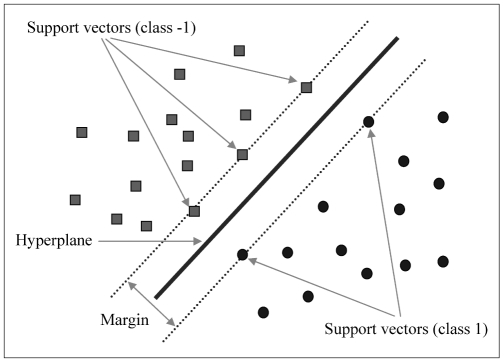
\includegraphics[width=0.5\linewidth]{figures/svm}
	\caption{A Support Vector Machine \parencite{svm_pic}}
	\label{fig:svm}
\end{figure}

This is all better understood with some visualization. 
Please take a look at \autoref{fig:svm}.
It is easy to see in this picture that the hyperplane is positioned to maximize the margin between the support vectors.
It is also important to realize that the data points that are not support vectors do not affect the hyperplane in any way. \parencite{homl:5}

Support vector machines can also be used for regression.
This is also done by constructing a hyperplane.
However, the objective is reversed.
This hyperplane is positioned to include as many data points in the margin as possible.
The size of the margin is determined by hyperparameter $\epsilon$. \parencite{homl:5}

For the mathematical background and more information on support vector machines, please refer to \parencite{homl:5}.

\subsubsection{Decision Trees}
Decision trees are a form of graph based models.\parencite{ml:prml}
More specifically, decision trees are trees that contain basic conditional statements on their non-leaf nodes.
For any given feature vector, a decision tree runs tests these conditions to reach a decision.
These tests start at the root of the tree.
Depending on the outcome of the test, a child node is selected.
This process continues iteratively until a leaf node is reached, where a decision is stored.
Decision in this context is the label for the feature vector.\parencite{ai:ml}


For the mathematical background and more information on decision trees, please refer to \parencite{homl:6}.

\subsubsection{Ensemble Learning}
Instead of training a singular model, we can train many weak models and aggregate the results.
Such aggregations of models are called ensembles, and the learning process is called ensemble learning.
One simple yet particularly powerful example is the random forest:
A random forest is an ensemble of decision trees, each trained on different random subsets of the training set.
A random forest makes predictions by aggregating the predictions of each individual tree.
For regression, the predictions are averaged.
For classification, the most predicted class is the final prediction.\parencite{homl:7}
 
More information on ensemble learning can be found at \parencite{homl:7}

\subsection{More Machine Learning}
Finally, let's go through some more advanced machine learning concepts that will be relevant in the next chapter.
\subsubsection{Data Preprocessing}
It is often the case that we have to work on imperfect data.
Some values might be missing for some instances, data might not be uniform or features might not be helpful as they are.
Collection of transformations we apply to the data before feeding it into to our models is called preprocessing.\parencite{homl:2}
This preprocessing includes:

Cleaning the data to make sure it is uniform.

Extracting features from the existing input variables.

Scaling the features to make sure all the features have similar scales.

The reasoning behind these transformations and more information on preprocessing can be found in \parencite{homl:2}.

\subsubsection{Cross Validation}
Cross validation is a technique used in model selection.
The data is first divided into $N$ parts.
Afterwards the model is trained on $N-1$ parts and validated on the remaining part.
This process is repeated $N$ times, each with a different part as the validation set.
Finally, the best performing model is selected.\parencite{ml:prml}
\subsubsection{Hyperparameter Optimization}
Hyperparameter optimization refers to the process of fine tuning the model hyperparameters to improve performance.
This is usually done automatically using grid-search.\parencite{homl:2} 

\subsubsection{$R^2$ Score}
$R^2$ Score (pronounced R squared) or the coefficient of determination is statistical metric.
In most simple terms, $R^2$ score shows how much of the variance in the target values can be explained by a statistical model.
It can be used to evaluate models, where a higher score indicates a better fit on data.
Best possible $R^2$ score is 1.0.
$R^2$ score can be negative too, indicating that the model is arbitrarily worse.\parencite{r2score}


\section{Nutrition}
\subsection{Dietary Assessment}
Food and Agriculture Organization of United Nations defines dietary assessment as the following:

``Dietary assessment is an evaluation of food and nutrient intake and dietary pattern of an individual or individuals in the household or population group over time.''
\parencite{faoun}

There are many different dietary assessment methods available, but we will be focusing on integration of innovative technologies to improve dietary assessment.
We will specifically be focusing on mobile-based technologies.
Mobile-based technologies allow users to log their dietary-intake in real time using a smartphone or a tablet.
This allows for higher quality control of the data.\parencite{faoun}
\subsection{Dietary Goals}
We couldn't find any resource that shows a collection of dietary goals that are collectively agreed upon by nutrition scientist.
However, popular dietary health applications such as MyFitnessPal and Fitbit implement three main dietary goals:

Lose weight

Maintain weight

Gain weight

After consulting S. Holzmann and B. Kaiser (personal communication, May 16, 2019), we have determined that this set of goals is also suitable for our task.
